\documentclass[12pt]{article}
\usepackage[margin=1.0in]{geometry} %page layout
\usepackage[usenames,dvipsnames]{color} %color
\definecolor{light-gray}{gray}{0.95}
\definecolor{darkgreen}{rgb}{0,0.4,0}
\usepackage{graphicx, subfigure} %figures
\usepackage{url, hyperref} %cross-referencing
\usepackage{amsmath, amssymb} %math
\usepackage{listings} %source code
\lstset{breaklines=true,
breakindent=0pt,
prebreak=\mbox{\tiny$\searrow$},
postbreak=\mbox{{\color{blue}\tiny$\rightarrow$}},
numbers=left,
commentstyle=\color{darkgreen},
numberblanklines=false,
frame=single,
captionpos=b,
backgroundcolor=\color{light-gray}}
\usepackage[3D]{movie15} %for movies (needs hyperref)
	\newenvironment{changemargin}[2]
	{
	  	\begin{list}{}
		{
			\setlength{\topsep}{0pt}%
			\setlength{\leftmargin}{#1}%
			\setlength{\rightmargin}{#2}%
			\setlength{\listparindent}{\parindent}%
			\setlength{\itemindent}{\parindent}%
			\setlength{\parsep}{\parskip}%
		}
	  	\item[]
		}
		{\end{list}
	}
\author{Salman Aslam\\Georgia Tech}
\title{Principal Components Analysis}
\date{}
\begin{document}
\maketitle
\rule[0pt]{\textwidth}{1pt}
\tableofcontents
\rule[0pt]{\textwidth}{1pt}

%===============================
\section{PCA}
%===============================
%------------------------------------------------------------------
\subsection{Introduction}
%------------------------------------------------------------------

One of the most critical failings of PCA is that translating points by arbitrary amounts inside the principal subspace has no effect on the model error~\cite{1999_JNL_Gaussian_roweis}.


\begin{itemize}
\item PCA assigns a low reconstruction cost to data points that are close to the principal subspace even if they lie arbitrarily far from the training data.
\end{itemize}

%------------------------------------------------------------------
\subsection{Theory}
%------------------------------------------------------------------

\subsubsection{Geometric derivation}
%-------------------------------------------


                \begin{figure}
                \centering
                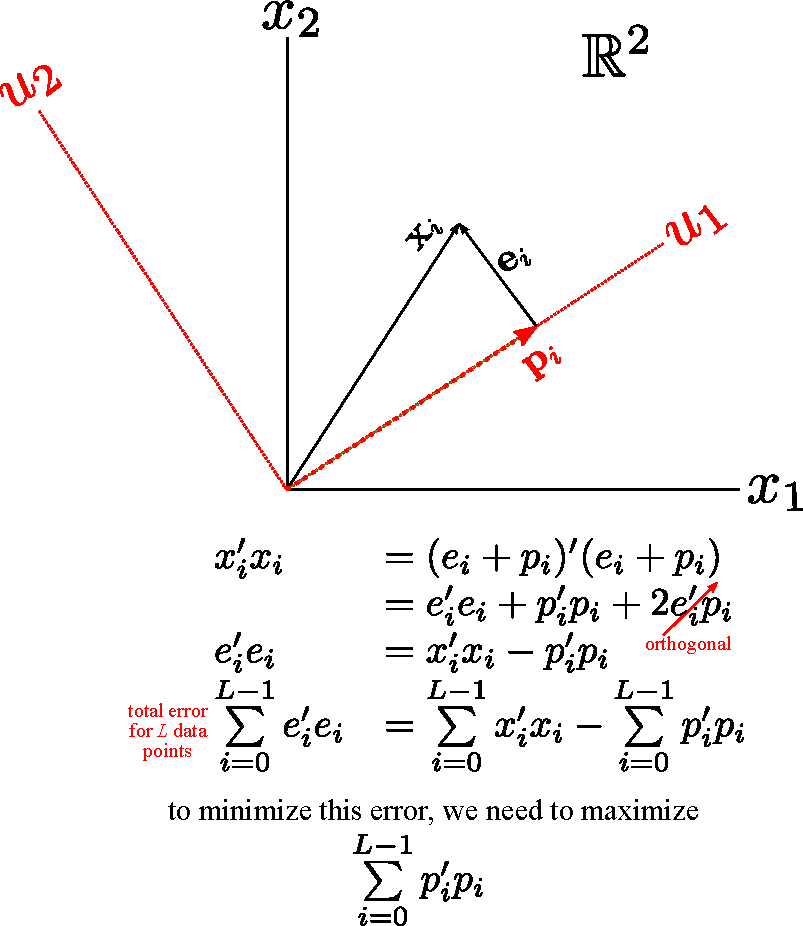
\includegraphics[width=0.6\textwidth]{figs/PRML_PCA_geometricDerivation_step1.pdf}
                \caption{PCA in $\mathbb{R}^2$.} 
                \label{fig:PCA_geometric1}
                \end{figure}



\subsubsection{Algebraic derivation}
%-------------------------------------------
\begin{equation}
\begin{array}{lllll}
&\mathbf{x}_i^T\mathbf{x}_i 										&= (\mathbf{e}_i + \mathbf{p}_i)^T(\mathbf{e}_i + \mathbf{p}_i) \\
&																		&=	\mathbf{e}_i^T\mathbf{e}_i + \mathbf{p}_i^T\mathbf{p}_i + 2\mathbf{e}_i^T\mathbf{p}_i\\
\Rightarrow&\mathbf{e}_i^T\mathbf{e}_i							&=	\mathbf{x}_i^T\mathbf{x}_i - \mathbf{p}_i^T\mathbf{p}_i\\
\Rightarrow&\sum\limits_{i=1}^N\mathbf{e}_i^T\mathbf{e}_i	&=	\sum\limits_{i=1}^N\mathbf{x}_i^T\mathbf{x}_i - \sum\limits_{i=1}^N\mathbf{p}_i^T\mathbf{p}_i
\end{array}
\label{Eqn:PCA_basic}
\end{equation}

Here, $\mathbf{e}_i^T\mathbf{p}_i=0$ since each $\mathbf{p}_i$ is orthogonal to its $\mathbf{e}_i$.  From Equation~\ref{Eqn:PCA_basic}, it is clear that in order to minimize $\mathbf{e}_i^T\mathbf{e}_i$, we need to maximize $\sum\limits_{i=1}^{N}\mathbf{p}_i^T\mathbf{p}_i$.  We now write,

\begin{equation}
\begin{array}{ll}
\sum\limits_{i=1}^N \mathbf{p}_i^T\mathbf{p}_i 				&= \sum\limits_{i=1}^N \mbox{tr}(\mathbf{p}_i\mathbf{p}_i^T)\\
				&= \sum\limits_{i=1}^N \mbox{tr}(\mathbf{U}_q^T\mathbf{x}\mathbf{x}^T\mathbf{U}_q)\\
				&= \mbox{tr} \left[ \mathbf{U}_q^T \left(\sum\limits_{i=1}^N (\mathbf{x}\mathbf{x}^T)\right) \mathbf{U}_q \right]\\
				&= \mbox{tr} (\mathbf{U}_q^T\mathbf{X}\mathbf{X}^T\mathbf{U}_q)\\
				&= \mbox{tr} (\mathbf{U}_q^T\Sigma \mathbf{U}_q)\\
				&= \mbox{tr} (\sum\limits_{i=1}^N \lambda_j \mathbf{u}_j \mathbf{u}_j^T)\\
				&= \sum\limits_{i=1}^N \lambda_j \mathbf{u}_j^T \mathbf{u}_j\\
\end{array}
\end{equation}


%===============================
\section{PPCA (Probabilistic PCA)}
%===============================
%------------------------------------------------------------------
\subsection{Introduction}
%------------------------------------------------------------------
In probabilistic PCA, or PPCA~\cite{1999_JNL_PPCA_Tipping}, the prinicipal axes of a set of $N$ observed vectors can be determined through maximum likelihood estimation of a set of parameters in a latent variable model closely tied to factor anlaysis.  The principal axes can also be determined using regular PCA and incorporated into the model.  As a result, incremental PCA (IPCA) is important here since it can be used to reduce the computational load in online situations.  But a natural question arises, if the principal axes can be computed using conventional means, what advantage does the probabilistic model give.  A probabilistic model allows comparison with other probabilistic models, allows statistical testing, permits application of Bayesian methods, and facilitates mixture models and general Gaussian density models.  Furthermore, the missing data problem can be effectively addressed in the resulting generative framework.  

%------------------------------------------------------------------
\subsection{Theory}
%------------------------------------------------------------------
We start by assuming that we have an observation vector $\mathbf{x} \in \mathbb{R}^D$.  Suspecting some correlation in the data, we believe that we can get a more parsimonious explanation of the dependencies between the observations using a \emph{latent}, i.e. hidden, variable  $\mathbf{z} \in \mathbb{R}^M, M<D$.  We model this variable with Gaussian prior distribution $p(\mathbf{z}) \sim \mathcal{N}(0, \mathbf{I})$.  The primary goal of latent variables is to allow a complicated distribution over the observed variables to be represented in terms of a model constructed from simpler (typically exponential family) conditional distributions.
The following model is proposed,

\begin{equation}
\boxed{
\mathbf{x}_{ \textrm{\tiny \emph{D}x1}} = \mathbf{W}_{ \textrm{\tiny \emph{D}x\emph{P}}}\mathbf{z}_{ \textrm{\tiny \emph{P}x1}}+ \mathbf{\mu}_{ \textrm{\tiny \emph{D}x1}} + \mathbf{\epsilon}_{ \textrm{\tiny \emph{D}x1}}}
\end{equation}

Here, $\mathbf{\mu}$ is the mean of the observations.  We are left to estimating the values of $\mathbf{W}$ and $\mathbf{\epsilon}$.  $\mathbf{\epsilon}$ is modeled as a gaussian random variable with zero mean and diagonal covariance matrix.  In PPCA, all entries on the diagonal are modeled as being exactly the same, i.e. an \emph{isotropic error model} is used, while in factor analysis, the entries on the diagonal are assumed to be different. Mathematically,

\begin{equation}
\begin{array}{lllll}
\textrm{PPCA} 				&:  \mathbf{\epsilon}\sim \mathcal{N}(\mathbf{0},\sigma^2 \mathbf{I})\\
\textrm{factor analysis} 	&:  \mathbf{\epsilon}\sim \mathcal{N}(\mathbf{0},\mathbf{\Psi})
\end{array}
\end{equation}

This is the \emph{only} difference between PPCA and factor analysis.  Naturally though, it affects the maximum likelihood computations that follow.  Since we are interested in PPCA, we will continue with modeling $\mathbf{\epsilon}$ using an isotropic error model.  For factor analysis, please refer to~\cite{2007_BOOK_PRML_Bishop} for more details.  

Under PPCA, the Gaussian conditional distribution $p(\mathbf{x}|\mathbf{z})$ is given by

\begin{equation}
p(\mathbf{x|z}) \sim \mathcal{N}(\mathbf{Wz} + \mathbf{\mu}, \sigma^2\mathbf{I})
\end{equation}

$\mathbf{x}_i$ are conditionally independent given the values of the latent variables $\mathbb{z}$.




                \begin{figure}
                \centering
                \includegraphics[width=0.6\textwidth]{figs/SP_covarianceSpectrum.pdf}
                \caption{Covariance matrix spectrum.  If the training set size $N$ is larger than the dimensionality of the data $D$, it is possible to model the data with a full covariance matrix.} 
                \label{fig:covariance_matrix_spectrum}
                \end{figure}


If we define a joint distribution over observed and latent variables, the corresponding distribution of the observed variables alone is obtained by marginalization.  This allows relatively complex marginal distributions over observed variables to be expressed in terms of more tractable joint distributions over the expanded space of observed and latent variables.  The introduction of latent variables thereby allows complicated distributions to be formed from simpler components.  



								\begin{table}[t]
								\centering
								\begin{tabular}{| l | c | c | l |}\hline
								\textbf{Name} & \textbf{Notation} & \textbf{Distribution} & \textbf{Remarks}\\\hline
								latent variable (factors) & $\mathbf{z} \in R^M$ & $ \mathcal{N}(\mathbf{0},\mathbf{I})$ & \parbox{2in}{iid, Gaussian variables with unit variance}\\\hline
								- & $ \mathbf{\epsilon}$ & $ \mathcal{N}(\mathbf{0},\sigma^2\mathbf{I})$ &-\\\hline
								- & $\mathbf{x|z} $ & $ \mathcal{N}(\mathbf{Wz+\mu},\sigma^2\mathbf{I})$ &-\\\hline              
								observations & $\mathbf{x} \in R^D$ & $ \mathcal{N}(\mathbf{\mu},\mathbf{WW}^T + \sigma^2\mathbf{I})$ &$D>M$ \\\hline
								\end{tabular}
								\caption{Notation}
								\end{table}



					                \begin{figure}[t]
					                \centering
					                \fbox{\includegraphics[width=0.5\textwidth]{figs/SP_covarianceSpectrum.pdf}}
					                \caption{Covariance matrix spectrum.  If the training set size $N$ is larger than the dimensionality of the data $D$, it is possible to model the data with a full covariance matrix.} 
					                \label{fig:covariance_matrix_spectrum}
					                \end{figure}

The latent variables explain the correlations between observation variables while $\psi_i$ represents variability unique to a particular $t_i$.




The likelihood function is,

\begin{equation}
\begin{array}{lllll}
p(\mathbf{x}|\mathbf{\mu, W}, \sigma^2) &= \frac{1}{(2\pi)^{D/2}|\Sigma|^{1/2}}e^{-\frac{1}{2}(\mathbf{x}-\mathbf{\mu})^T\Sigma^{-1}(\mathbf{x}-\mathbf{\mu})}\\
&= \frac{1}{(2\pi)^{D/2}|\Sigma|^{1/2}}e^{-\frac{1}{2}(\mathbf{x}-\mathbf{\mu})^T(\mathbf{W}\mathbf{W}^T + \sigma^2 \mathbf{I})^{-1}(\mathbf{x}-\mathbf{\mu})}\\
\end{array}
\end{equation}

The log likelihood function is,

\begin{equation}
\begin{array}{lllll}
\ln p(\mathbf{x}|\mathbf{\mu, W}, \sigma^2) &= -\frac{D}{2}\ln 2\pi -\frac{1}{2} \ln |\Sigma| -\frac{1}{2}(\mathbf{x}-\mathbf{\mu})^T(\mathbf{W}\mathbf{W}^T + \sigma^2 \mathbf{I})^{-1}(\mathbf{x}-\mathbf{\mu})
\end{array}
\end{equation}



The data covariance matrix $\mathbf{S}$ is,

\begin{equation}
\mathbf{S} = \frac{1}{N} \sum\limits_{n=1}^N (\mathbf{x}_n - \bar{\mathbf{x}})(\mathbf{x}_n - \bar{\mathbf{x}})^T
\end{equation}

The maximum likelihood estimate for the mean $\mathbf{\mu}$ is,

\begin{equation}
\boxed{
\mathbf{\mu}^* = \mathbf{\bar{x}}}
\end{equation}

The maximum likelihood estimate for $\mathbf{W}$ is,

\begin{equation}
\boxed{
\mathbf{W}^* = \mathbf{U}_{ \textrm{\tiny \emph{D}x\emph{P}}}(\mathbf{L}_{ \textrm{\tiny \emph{P}x\emph{P}}} - \sigma^2\mathbf{I}_{ \textrm{\tiny \emph{P}x\emph{P}}})^{1/2}\mathbf{R}_{ \textrm{\tiny \emph{P}x\emph{P}}}}
\end{equation}


Here, $\mathbf{U}_{ \textrm{\tiny \emph{D}x\emph{P}}}$ is created from an arbitrary set of $P$ eigenvectors of the data covariance matrix $\mathbf{S}$, $\mathbf{L}_{ \textrm{\tiny \emph{P}x\emph{P}}}$ has the corresponding eigenvalues $\lambda_i$, and $\mathbf{R}_{ \textrm{\tiny \emph{P}x\emph{P}}}$ is an arbitrary orthogonal matrix.

Finally, the maximum likelihood for the variance $\sigma^2$ is,
\begin{equation}
\boxed{
{\sigma^*}^2 = \frac{1}{D-P}\sum\limits_{i=P+1}^D \lambda_i}
\end{equation}


%------------------------------------------------------------------
\subsection{Experiments}
%------------------------------------------------------------------

%------------------------------------------------------------------
\subsection{Results}
%------------------------------------------------------------------

%------------------------------------------------------------------
\subsection{Conclusions}
%------------------------------------------------------------------

%------------------------------------------------------------------
\subsection{Source code}
%------------------------------------------------------------------
\scriptsize
\lstinputlisting[language=Matlab, caption={demo\_PPCA.m.}, 									label=lst:demo_PPCA]									{demo_PPCA.m}
\normalsize

%===============================
\section{IPCA (Incremental PCA)}
%===============================
In incremental PCA, or IPCA, the goal is to compute an incremental basis as data becomes available online.  This can be done using an incremental SVD procedure.  Refer to the report on incremental SVD for more details.

%===============================
\section{KPCA (Kernel PCA, to do)}
%===============================
Kernel PCA, or KPCA, is a method in which dimensionality reduction is applied after applying the kernel "trick" to the data.

%===============================
\section{Relationship between PCA and K-means (to do)}
%===============================
Refer to the brilliant work by Ding and He, 2004~\cite{2004_CNF_KmeansVsPCA_DingHe}.  They have tied together the workhorse of machine learning, PCA, with the workhorse of signal processing, K-means.  I am going to write about this in detail, eventually :)

\bibliographystyle{ieee}
\bibliography{MyCitations}
\end{document}


%$\Rightarrow \mathsf{t}\sim \mathcal{N}(\mathbf{\mu},\mathbf{WW^T\Psi})$.




